          % Rects 
          %\documentclass[tikz,border=5]{standalone}
          %\begin{document}
          %\begin{tikzpicture}
          %\foreach \i [evaluate={\ii=int(\i-1);}] in {0,...,11}{
          %  \foreach \j [evaluate={\jj=int(\j-1);}] in {0,...,11}{
          %    \coordinate [shift={(\j,\i)}] (n-\i-\j) at (rand*180:1/4+rnd/8);
          %\ifnum\i>0
          %  \draw [help lines] (n-\i-\j) -- (n-\ii-\j);
          %\fi
          %\ifnum\j>0
          %  \draw [help lines] (n-\i-\j) -- (n-\i-\jj);
          %\fi
          %}}
          %\end{tikzpicture}
          %\end{document}


          % And some triangles...

          \documentclass[tikz,border=5]{standalone}
          \begin{document}
          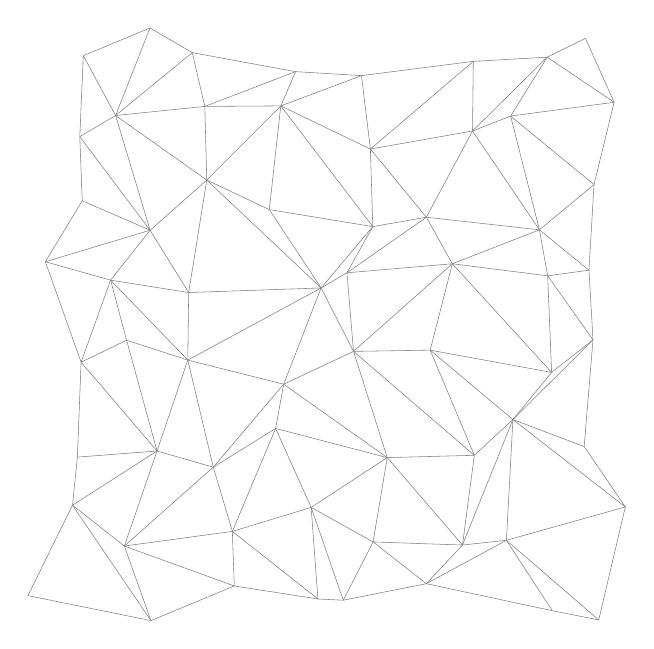
\begin{tikzpicture}
          \foreach \i [evaluate={\ii=int(\i-1);}] in {0,...,7}{
            \foreach \j [evaluate={\jj=int(\j-1);}] in {0,...,7}{
              \coordinate [shift={(\j,\i)}] (n-\i-\j) at (rand*180:1/4+rnd/8);
          \ifnum\i>0
            \draw [help lines] (n-\i-\j) -- (n-\ii-\j);
          \fi
          \ifnum\j>0
            \draw [help lines] (n-\i-\j) -- (n-\i-\jj);
            \ifnum\i>0
              \pgfmathparse{int(rnd>.5)}
              \ifnum\pgfmathresult=0
                \draw [help lines] (n-\i-\j) -- (n-\ii-\jj);
              \else%
                \draw [help lines] (n-\ii-\j) -- (n-\i-\jj);
              \fi%
            \fi
          \fi
          }}
          \end{tikzpicture}
          \end{document}
